% =========================================================================
% CAPITOLO 8 — VALUTARE: LO STUDIO CON UTENTI
% =========================================================================

\chapter{Studio con utenti}
\label{ch:userstudy}

\noindent
{\rmfamily\itshape
\begin{tabular}[t]{@{}l@{\hspace{0.3cm}}p{12.5cm}@{}}
\textls[50]{\textbf{Trattati:}} &
\textls[50]{Test e validazione · Disegno tra soggetti · Strumento del questionario · Protocollo
di comprensione scritta · Quadro di codifica · Consenso ed etica · Limiti del disegno}
\end{tabular}
}

\vspace{0.5cm}

Il Capitolo~\ref{ch:translate} ha sviluppato l'artefatto e ha mostrato che le due condizioni sono allineate per provenienza, inquadramento e unità di misura, differendo deliberatamente in un aspetto: la condizione esperienziale porta la dimensione temporale che quella statica trattiene, che è la variabile che lo studio si propone di esaminare. La domanda successiva è se presentarla in modi diversi incida su come le persone la comprendono. Lo studio non mira a dimostrare che la visualizzazione esperienziale sia migliore; esamina se un piccolo gruppo di partecipanti per lo più non specialisti comprenda il sistema in modo diverso sotto una visualizzazione statica o una esperienziale, ed è progettato così che tanto risultati positivi quanto negativi informino lo stadio successivo. È uno \emph{studio socio-cognitivo}, rivolto a come le persone interpretano le visualizzazioni anziché a testare la scienza sottostante o la competenza dei partecipanti.

% -------------------------------------------------------------------------
\section{Scopo}
\label{sec:eval-purpose}

I Capitoli~\ref{ch:data_pipeline} e~\ref{ch:translate} hanno affrontato rilevamento e traduzione. Il passo restante era mettere le due forme di rappresentazione davanti ai partecipanti e confrontare come vengono comprese --- ciò che la domanda di ricerca centrale (\S\ref{sec:rqs}) chiede --- perciò era richiesto uno \emph{studio comparativo con utenti}. Poiché le visualizzazioni animate possono apparire più efficaci semplicemente perché portano informazione che la versione statica non ha \citep{tversky2002}, lo studio allinea le due condizioni per provenienza, inquadramento e unità di misura e varia solo la forma.

% -------------------------------------------------------------------------
\section{Un primo stadio esplorativo}
\label{sec:eval-exploratory}

Lo studio è esplorativo per disegno. Hanno partecipato venticinque persone, dodici assegnate alla condizione statica e tredici all'esperienziale.\footnote{La differenza tra dodici e tredici deriva dall'assegnazione casuale a una piccola dimensione campionaria. Non incide su nulla nell'analisi descrittiva oltre i denominatori usati nel Capitolo~\ref{ch:results}.}

La dimensione campionaria è stata fissata a priori, su basi di fattibilità e dell'obiettivo esplorativo. Un criterio di saturazione non è rivendicato e non si adatterebbe: la saturazione appartiene ai disegni induttivi e generativi di teoria, mentre questa analisi è deduttiva rispetto a una griglia fissata prima di leggere le risposte \citep{braunclarke2021}.

Il criterio difendibile è l'\emph{information power} \citep{malterud2016}: uno studio qualitativo ha bisogno di meno partecipanti man mano che il suo obiettivo si restringe, il suo campione si fa più specifico, il suo fondamento si rafforza e la sua analisi lavora per categorie. Questo studio è ristretto nell'obiettivo, specifico nel campione, fondato sulla griglia di codifica del Capitolo~\ref{ch:literature} e analizzato per categoria --- una configurazione per cui venticinque partecipanti portano adeguata information power, e nessuna per l'inferenza su scala di popolazione che lo studio non tenta.

Questo primo studio individua invece pattern iniziali per la ricerca futura: quali concetti i partecipanti comprendono, quali sono comunemente fraintesi, se le due condizioni sembrino portare a interpretazioni diverse, e se l'approccio sia abbastanza promettente da giustificare uno studio più ampio e statisticamente potente.

% -------------------------------------------------------------------------
\section{Partecipanti e pubblico}
\label{sec:eval-audience}

Lo studio si rivolgeva a non specialisti: partecipanti senza formazione specifica in oceanografia, scienza del clima, matematica o machine learning. Lo status di non specialista è stato stabilito per auto-dichiarazione nella sezione di background. Ciò riflette l'obiettivo della tesi: le visualizzazioni sono intese a sostenere la comprensione di sistemi complessi oltre il pubblico specializzato.

Non ci si aspettava che i partecipanti avessero conoscenza pregressa dell'AMOC o dei concetti usati nelle visualizzazioni; il questionario forniva l'informazione di base necessaria ad affrontare le scene. Il reclutamento è avvenuto attraverso reti personali in italiano e in inglese, perciò il campione è di convenienza: la sua composizione è descritta nella \S\ref{sec:res-sample} e le sue implicazioni nella \S\ref{sec:eval-limitations}.

% -------------------------------------------------------------------------
\section{Lo strumento}
\label{sec:eval-instrument}

Lo studio è stato condotto come questionario scritto autoguidato tramite Google Forms. Sono state usate quattro versioni del questionario, combinando due lingue (italiano e inglese) con le due condizioni sperimentali (statica ed esperienziale).\footnote{Le quattro versioni usano la stessa formulazione entro ciascuna lingua e differiscono solo nei link alle scene che conducono alle visualizzazioni statiche o esperienziali. I protocolli completi del questionario sono forniti nell'Appendice~\ref{app:protocols}.}

% it/figures/user_study/Google_Form.tex — versione italiana
\begin{figure}[htbp]
    \centering
    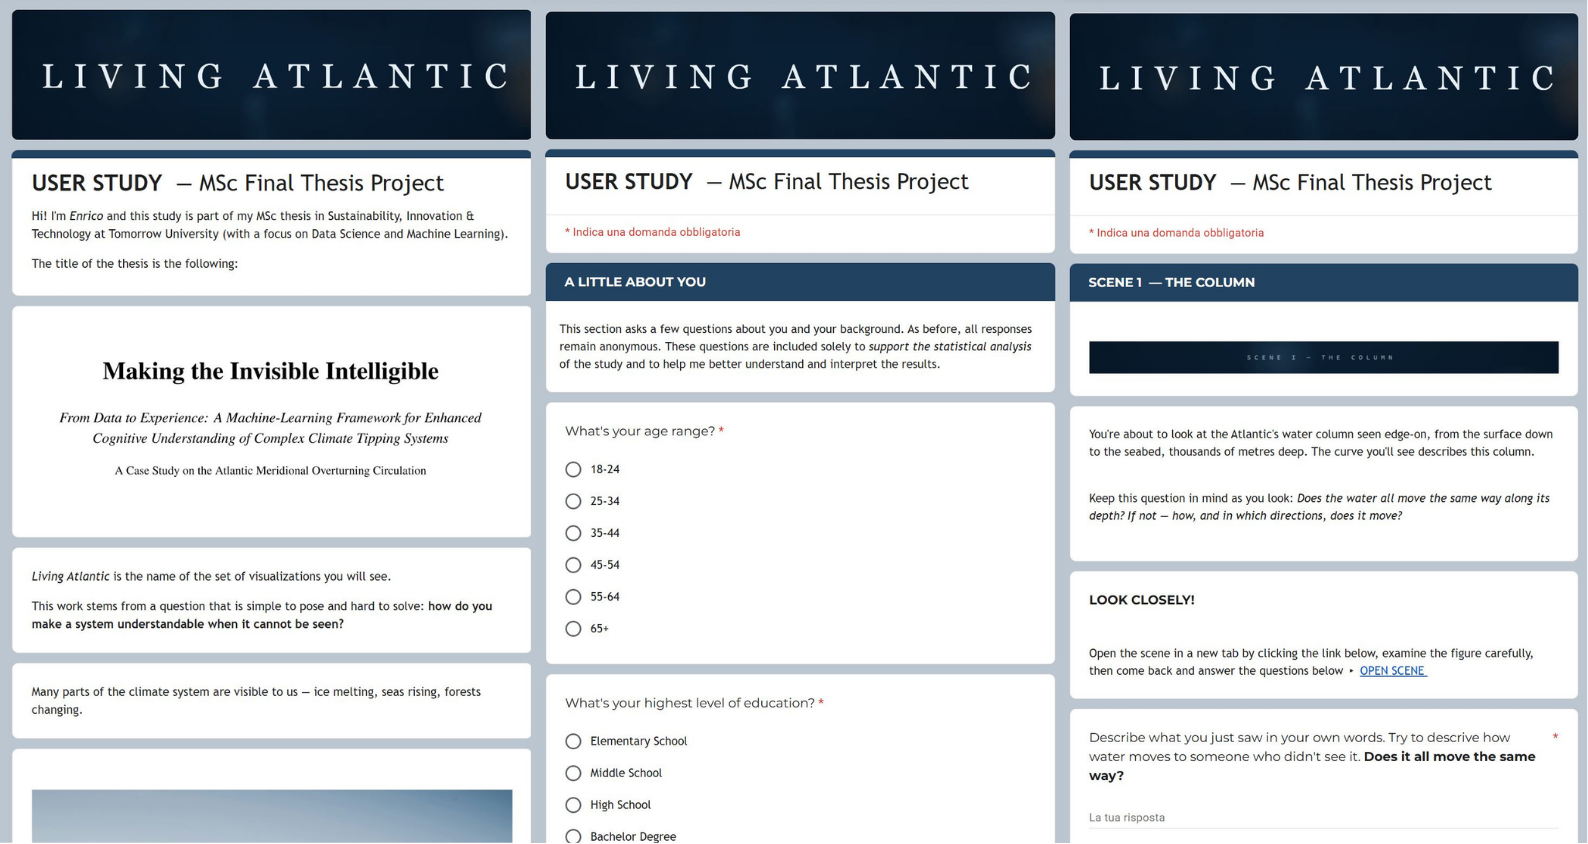
\includegraphics[width=\textwidth]{figures/user_study/Google_Form.png}
    \caption[Il questionario dello studio in Google Forms]{Il Google Form usato per la
    raccolta dati, che mostra l'introduzione, gli item di background e il blocco della
    prima scena. Il modulo raccoglieva descrizioni scritte di ciascuna scena e
    valutazioni di fiducia.}
    \label{fig:google-form}
\end{figure}


Un questionario scritto e auto-somministrato è stato preferito a un protocollo think-aloud con sessioni dal vivo: raggiunge più partecipanti e dà a tutti le stesse istruzioni senza che un intervistatore influenzi le risposte.

Il questionario segue un'unica sequenza: introduzione, consenso, informazioni sull'anonimato, una breve sezione di background e il contesto di base necessario a comprendere l'AMOC e lo sverdrup --- tutto identico per entrambi i gruppi. Le tre scene seguono poi in ordine (\textit{La colonna}, \textit{La sala macchine}, \textit{La soglia}). Per ciascuna, i partecipanti ricevono una breve introduzione e una domanda guida, aprono la visualizzazione assegnata, la esplorano e, al ritorno, rispondono a domande aperte con parole proprie. Una riflessione finale e un debriefing chiudono il questionario.

L'ordine delle domande è intenzionale: i partecipanti descrivono ciò che hanno compreso con parole proprie prima che sia chiesto loro di valutare la propria fiducia o di riflettere sull'esperienza, e la struttura a due condizioni è spiegata solo dopo che le risposte principali sono state raccolte.

% -------------------------------------------------------------------------
\section{Le condizioni dello studio}
\label{sec:eval-conditions}

I due gruppi differivano solo nel tipo di visualizzazione esperita. Entrambi hanno visto le stesse tre scene --- \textit{La colonna}, \textit{La sala macchine} e \textit{La soglia} --- con le stesse domande e le stesse informazioni contestuali; il gruppo di controllo ha visto ciascuna come visualizzazione statica convenzionale, il gruppo esperienziale come la sua controparte interattiva e dinamica.\footnote{Il disegno delle tre scene, e la distinzione tra le loro componenti derivate dal machine learning e quelle classiche, è descritto nella \S\ref{sec:three-scenes}. Il Capitolo~\ref{ch:translate} stabilisce che entrambe le condizioni usano lo stesso bundle di dati, la stessa funzione di ricostruzione e la stessa provenienza.}

Una precisazione conta: il machine learning non genera ogni elemento delle condizioni esperienziali --- il campo di particelle della Scena~I è una derivata, la dispersione della Scena~III viene da modelli oceanici esterni --- perciò lo studio confronta due modi di presentare lo stesso sistema, non una condizione di machine learning contro una non di machine learning.

% -------------------------------------------------------------------------
\section{Randomizzazione e debriefing}
\label{sec:eval-randomisation}

I partecipanti sono stati assegnati casualmente a una delle due condizioni. Con un piccolo campione, la randomizzazione non può garantire gruppi bilanciati, ma rimuove l'autoselezione in una condizione e così limita una fonte sistematica di bias. Ogni partecipante è rimasto nella condizione assegnata fino alla fine dello studio principale, così che l'esposizione all'alternativa non potesse influenzare le sue risposte.\footnote{Mantenere la struttura sperimentale non svelata fino alla fine riduce anche la possibilità che i partecipanti interpretino la propria esperienza come parte di un confronto e aggiustino di conseguenza le risposte.}

Una volta raccolte tutte le risposte principali, il debriefing ha spiegato la struttura, introdotto le due condizioni e dato a ogni partecipante accesso all'insieme completo delle visualizzazioni --- inclusa la versione che non aveva esperito.

% -------------------------------------------------------------------------
\section{Sezione di background}
\label{sec:eval-demographics}

Una breve sezione di background prima dei compiti ha raccolto fascia d'età, istruzione, ambito di studio o lavoro e familiarità auto-valutata con la scienza del clima, l'AMOC e le visualizzazioni di dati.

Il suo scopo è descrittivo: dato il piccolo campione, queste variabili descrivono il pubblico e inquadrano i risultati anziché alimentare una modellazione statistica.

% -------------------------------------------------------------------------
\section{Consenso, anonimato ed etica}
\label{sec:eval-ethics}

La partecipazione era volontaria e anonima: il questionario non ha raccolto nomi, indirizzi email o altri identificatori diretti, i partecipanti potevano interrompere in qualsiasi momento senza dare una ragione, e il consenso è stato ottenuto prima dell'inizio dello studio attraverso una conferma esplicita che proseguire significava accettare di partecipare. Le risposte sono state usate solo per questa ricerca, e nessuna informazione identificativa compare nel Capitolo~\ref{ch:results}. Il testo di consenso e anonimato è riprodotto nell'Appendice~\ref{app:protocols}; gli impegni etici che attua sono esposti nella \S\ref{sec:ethics-statement} e nell'Appendice~\ref{app:ethics-conduct}.

% -------------------------------------------------------------------------
\section{Quadro di valutazione}
\label{sec:eval-framework}

Le risposte aperte sono analizzate rispetto a una griglia di codifica predefinita. Lo scopo non è segnare le risposte come giuste o sbagliate ma identificare se i partecipanti esprimano l'idea strutturale principale che ciascuna scena rappresenta.\footnote{La griglia completa, incluso il target di ciascuna scena e la definizione di ciascuna categoria, è fornita nell'Appendice~\ref{app:protocols}.}

Le categorie sono state definite prima di analizzare le risposte, e ciascuna è legata alla domanda guida della sua scena (\S\ref{sec:three-scenes}): direzioni opposte a profondità diverse per la Scena~I, ricorrenza tra stati per la Scena~II, e cambiamento nel livello di accordo tra i tre modelli per la Scena~III. Una risposta conta come dimostrazione di comprensione solo quando il partecipante descrive la struttura rilevante con parole proprie; menzionare movimento, colore o altre caratteristiche visive non è sufficiente.

La codifica è stata svolta attraverso una procedura assistita. Un large language model, istruito sulla griglia di codifica e sulle definizioni delle categorie, ha prodotto un'etichetta iniziale per ciascuna risposta. Il ricercatore ha poi riesaminato ogni etichetta e l'ha corretta ovunque il proprio giudizio differisse dalla proposta automatica. La codifica finale è quindi il risultato di un'adjudicazione umana, con il passaggio automatico che funge solo da punto di partenza. In questo studio la revisione ha mantenuto ognuna delle 75 etichette del modello, perciò il tasso di override è stato nullo. Un accordo completo di questo tipo è coerente con una griglia chiara e ben specificata, ma di per sé non può essere separato dal rischio di ancoraggio che una procedura assistita comporta --- un revisore che vede prima l'etichetta proposta può confermarla anziché giudicarla da capo.\footnote{La griglia di codifica predefinita (Appendice~\ref{app:protocols}) è ciò che mantiene trasparente questa procedura: ogni etichetta può essere riverificata da altri usando i criteri fissi e le risposte originali. Non è riportato alcun coefficiente di accordo tra codificatori, poiché tale misura non si applica a un disegno a codificatore singolo supportato da un primo passaggio automatico. Il limite dell'analisi a codificatore singolo è discusso nella \S\ref{sec:eval-limitations}.}

Il quadro mantiene anche la comprensione dimostrata --- la descrizione scritta --- separata dalla comprensione percepita, la valutazione di fiducia, perché i partecipanti possono sentirsi sicuri anche quando la loro interpretazione non corrisponde alla struttura intesa.\footnote{\textcite{fischer2020} documenta casi in cui un'alta fiducia accompagna un'interpretazione errata. L'analisi quindi incrocia la fiducia con le risposte codificate anziché trattarla come prova di comprensione corretta.}

% -------------------------------------------------------------------------
\section{Cosa lo studio si aspetta di trovare}
\label{sec:eval-expectations}

Lo studio chiede se la condizione esperienziale sostenga una comprensione più chiara di quella statica, nei termini delle aspettative E3.1 ed E3.2 (\S\ref{sec:hypotheses}): se profondità e direzioni opposte diventino più facili da comprendere (Scena~I), la ricorrenza più facile da riconoscere (Scena~II), e i cambiamenti nell'accordo tra modelli più facili da percepire (Scena~III). Queste sono aspettative, non previsioni, e nessuna presume una direzione o un'entità dell'effetto.

% -------------------------------------------------------------------------
\section{Tempi e carico}
\label{sec:eval-burden}

Il questionario è stato progettato per richiedere da quindici a venti minuti: abbastanza breve da evitare affaticamento inutile, abbastanza lungo da esplorare tre visualizzazioni.

% -------------------------------------------------------------------------
\section{Limiti del disegno}
\label{sec:eval-limitations}

Lo studio ha diversi limiti importanti. Primo, il campione è piccolo (venticinque partecipanti) e leggermente sbilanciato (dodici statica, tredici esperienziale), e non fornisce potenza statistica sufficiente per un'analisi inferenziale forte o una generalizzazione su scala di popolazione.

Secondo, i partecipanti sono stati reclutati attraverso reti personali, rendendo il campione di convenienza. La sua età, il suo background e la sua esperienza possono quindi differire da quelli della più ampia popolazione che le visualizzazioni intendono in ultima analisi raggiungere.

Terzo, tutti i partecipanti hanno incontrato le tre scene nello stesso ordine fisso (I, II, III), scelto per le ragioni interpretative esposte nella \S\ref{sec:three-scenes}. Poiché quell'ordine non è stato controbilanciato, la posizione nella sequenza è confusa con l'identità della scena: qualsiasi confronto \emph{tra} scene porta un possibile contributo dall'apprendimento lungo la sequenza o dall'affaticamento verso la fine. Questo riguarda direttamente il risultato della Scena~III, dove la condizione esperienziale ha reso meno bene e dove il compito cadeva anche per ultimo in un questionario di quindici-venti minuti. Un secondo caveat specifico della Scena~III è che il briefing di controllo diceva ai partecipanti che la figura statica permetteva loro di ``vedere dove concordano e dove differiscono'', e l'item di comprensione (Q16) chiedeva direttamente se i tre modelli concordano o divergono nel tempo; entrambi possono aver suggerito la lettura di convergenza, offrendo un'ulteriore possibile ragione per cui la condizione di controllo ha raggiunto ogni partecipante. Controbilanciare l'ordine delle scene, e neutralizzare questi suggerimenti, è un requisito per qualsiasi replica più ampia.

Quarto, lo studio usa risposte scritte e auto-riportate. Ciò significa che l'analisi è limitata a ciò che i partecipanti sono in grado o disposti a esprimere per iscritto. Alcuni aspetti della comprensione possono quindi restare non osservati.

Quinto, le risposte sono state codificate da un singolo ricercatore con un primo passaggio automatico e senza un secondo codificatore indipendente, perciò non può essere riportata alcuna affidabilità tra codificatori e si applica il rischio di ancoraggio segnalato nella \S\ref{sec:eval-framework}. La griglia definita a priori mantiene ogni assegnazione aperta a una riverifica esterna rispetto a criteri fissi, ma non sostituisce una doppia codifica indipendente.

Sesto, le due condizioni pongono richieste diverse all'hardware del partecipante. La condizione esperienziale anima di continuo e riproduce audio in tempo reale, mentre quella statica no, perciò un dispositivo più lento degrada una condizione e non l'altra. Non sono state raccolte informazioni su dispositivo o browser, e questa asimmetria è quindi riconosciuta anziché controllata.

Settimo, il briefing condiviso della Scena~II descriveva il centro della nuvola di punti come lo stato a cui l'oceano ``tende naturalmente a tornare''. Questo anticipa la ricorrenza che la scena chiede ai partecipanti di notare ed è fisicamente impreciso --- il centro è la media del record, non un equilibrio dinamico verso cui il sistema è richiamato --- perciò in qualsiasi replica serve una formulazione neutra.

Infine, lo studio distingue tra comprensione dimostrata e percepita. Un partecipante può riportare alta fiducia senza mostrare la comprensione strutturale attesa nella sua risposta scritta. Ciò non è trattato come un errore metodologico, ma come una distinzione importante che il quadro di valutazione è progettato per catturare.

% (Google_Form.tex era qui, orfano dopo l'ultima sezione; ora sta in 8.4)
Questi limiti non tolgono valore allo studio: fornisce un primo test empirico dell'approccio e individua pattern per guidare una replica più ampia, più controllata e statisticamente potente --- una base empirica iniziale anziché una validazione finale.
